\documentclass{beamer}
\usepackage{ctex}
\usepackage{zhs}
\usepackage{diagbox}  % 斜线表头
\usepackage{colortbl} %
\title{python语言程序设计基础}
\author{Hengsheng Zhou}
\institute{电信与智能制造学院}
\begin{document}
\begin{frame}[t]
	\titlepage
	\begin{figure}
		\begin{center}
			\includegraphics[width=0.2\linewidth]{output.eps}
		\end{center}
	\end{figure}


\end{frame}
\begin{frame}
	\frametitle{Outline}
	\tableofcontents
\end{frame}
\section{说课}

\subsection{为什么学python}

\begin{frame}[t]
	1. Python 用途广泛,生态丰富,无论是初学者还是专业开发者,都能在不同领域找到合适的应用场景!
	\pause
	\begin{table}[h]
		\centering
		\begin{tabular}{|c|c|c|c|}
			\hline
			\diagbox{应用场景}{示例} & 框架                        \\
			\hline
			数据分析               & Matplotlib/Seaborn(数据可视化) \\
			\hline
			自动化                & 批量文件处理                    \\
			\hline
			数据采集               & Scrapy                    \\
			\hline
		\end{tabular}
	\end{table}
	\pause
	2. Python 语法简洁、易学易用,适合零基础入门.
	\pause
	\begin{center}
		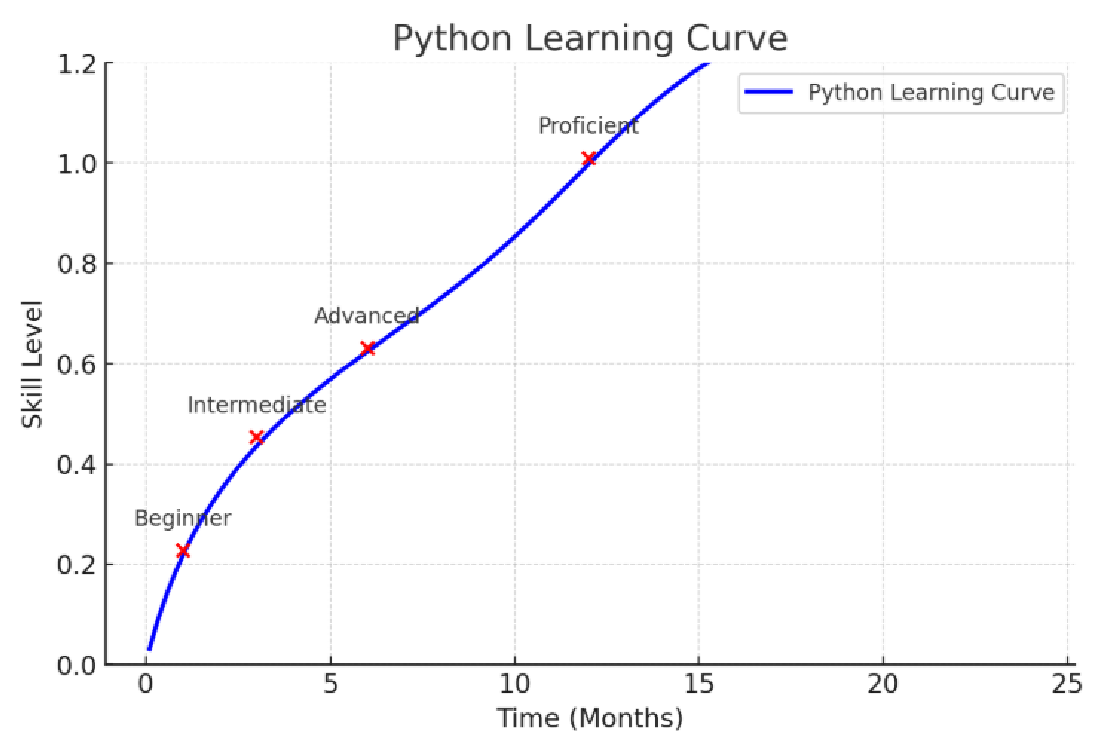
\includegraphics[width=0.5\linewidth]{learning_curve.eps}
	\end{center}

\end{frame}

\begin{frame}[t]
	\begin{center}
		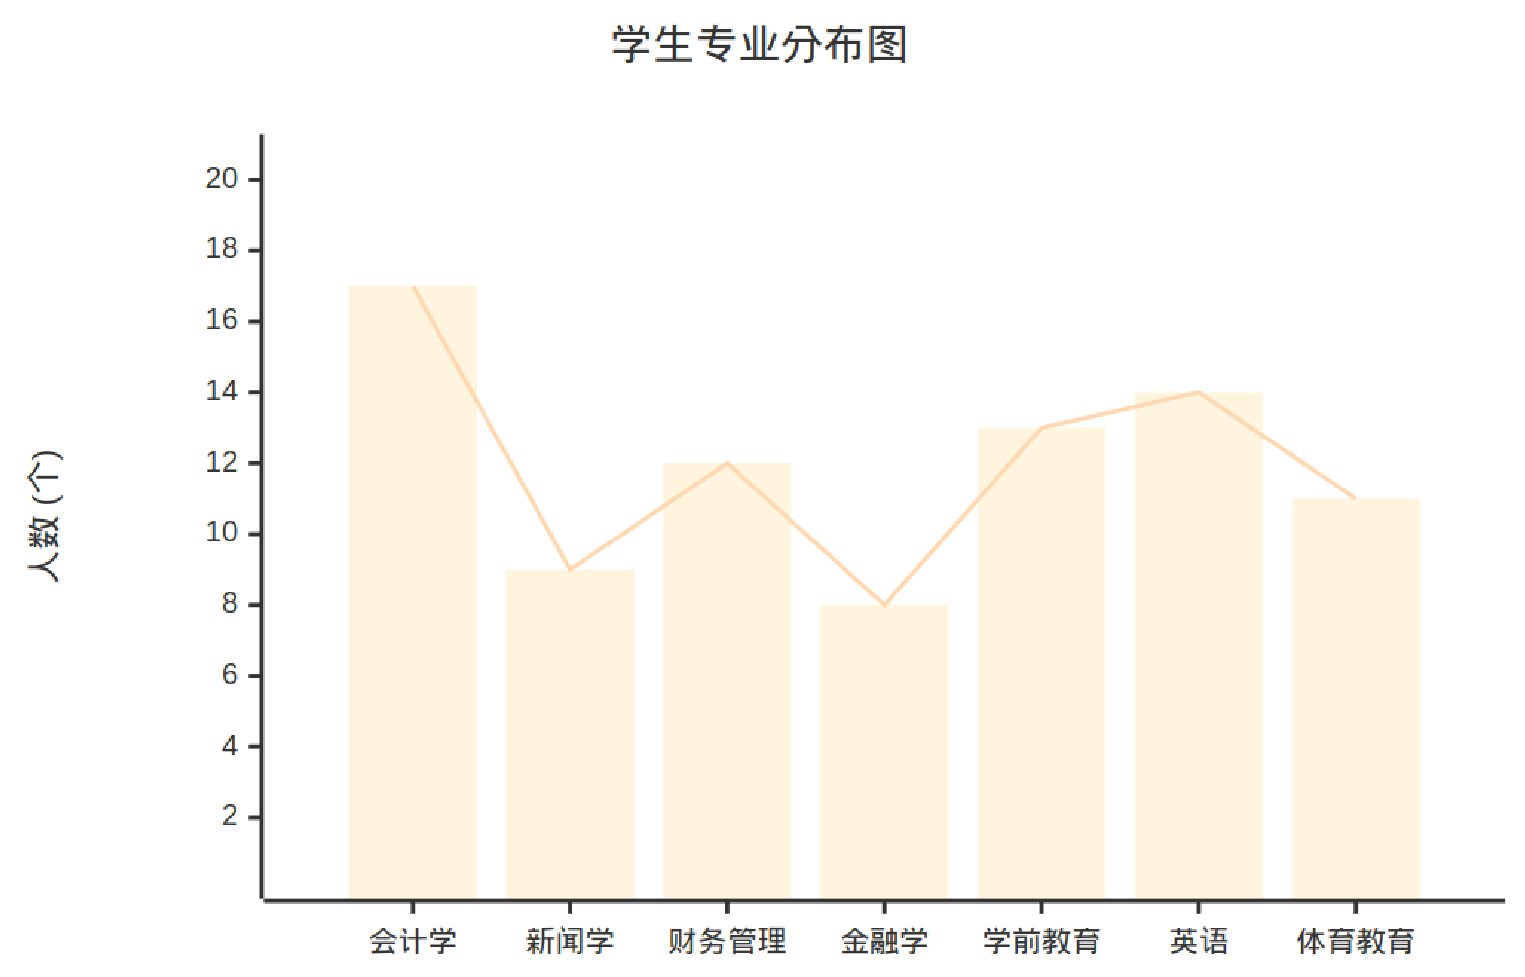
\includegraphics[width=0.6\linewidth]{student_number.eps}
	\end{center}
	\pause
	\begin{center}
		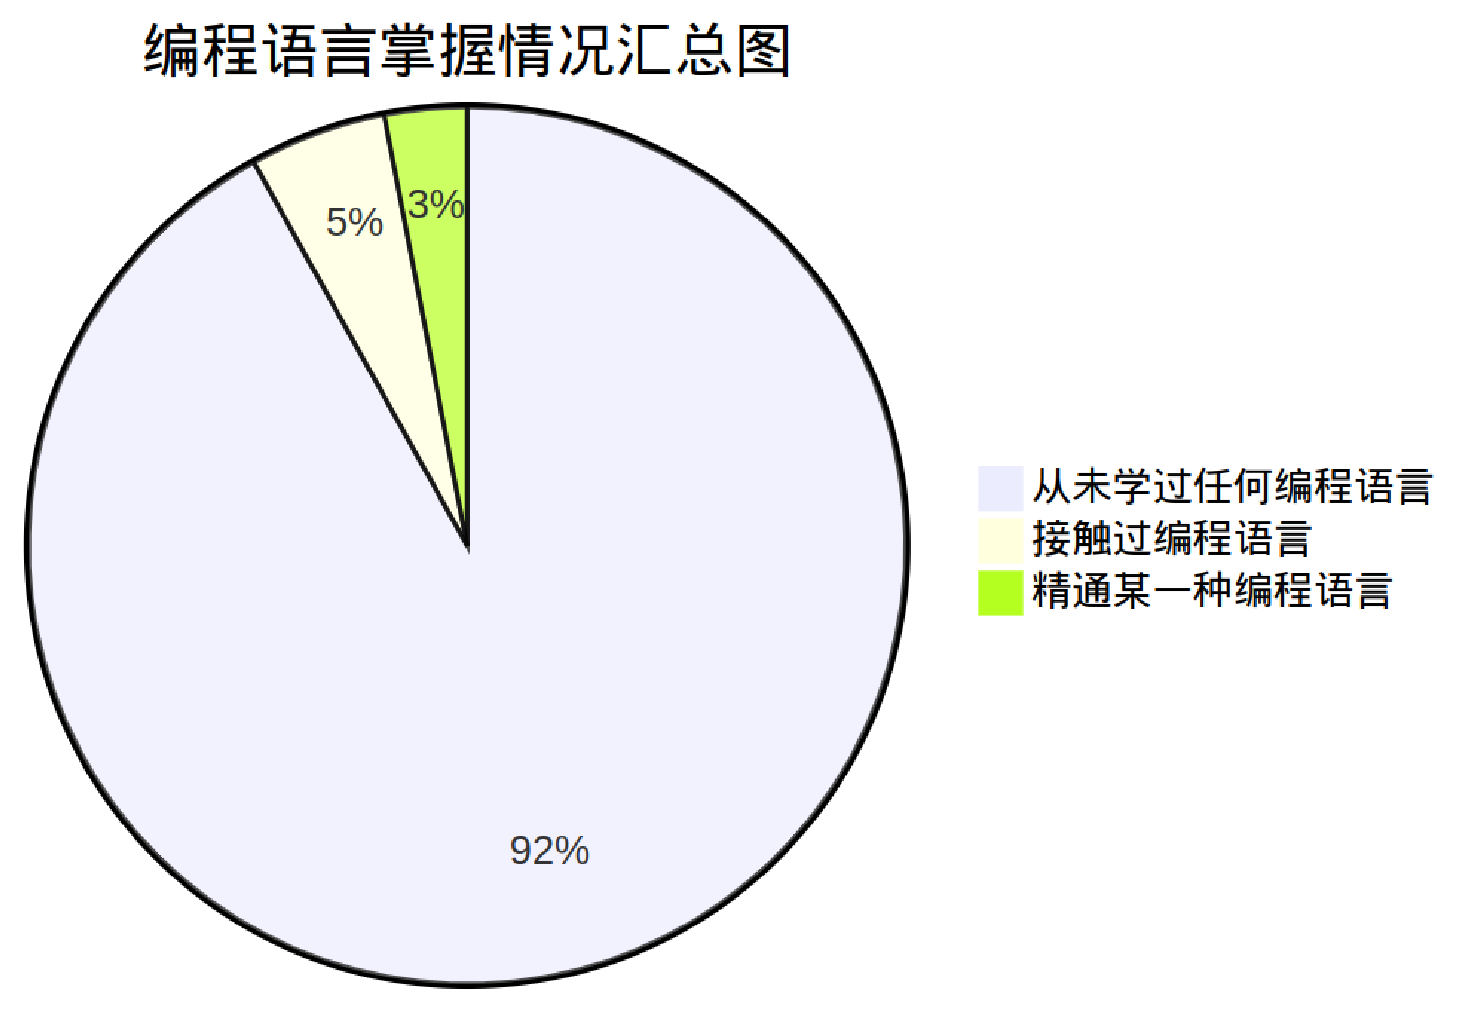
\includegraphics[width=0.4\linewidth]{pie.eps}
	\end{center}
\end{frame}


\subsection{怎么学}

\begin{frame}[t]
	\begin{itemize}
		\item<1-> 避免陷入“理论陷阱”
		      \pause
		      \begin{alertblock}{solution}
			      学一点就写代码,实践出真知,避免只看不练
		      \end{alertblock}
		      \pause
		\item<2-> 先掌握最基础的知识
		      \pause
		      \begin{alertblock}{solution}
			      遇到复杂的问题就先跳过,由浅入深
		      \end{alertblock}
		      \pause
		\item<3-> 熟练使用AI辅助工具
		      \pause
		      \begin{alertblock}{solution}
			      学会使用deepseek,chatGPT等AI辅助工具编写代码
		      \end{alertblock}
		      \pause
		\item<4-> 找python开发社区交流经验
		      \pause
		      \begin{alertblock}{solution}
			      学习在GitHub和Stack Overflow等开源社区寻找学习资源
		      \end{alertblock}



	\end{itemize}

\end{frame}

\subsection{课程思政}

\begin{frame}[t]
	在专业课程教学中融入思政教育,实现知识传授和价值引导的统一,是教学过程中不可或缺的重要环节,课程思政教育贯穿本课程教学全过程。
	\begin{figure}[htbp]
		\begin{center}
			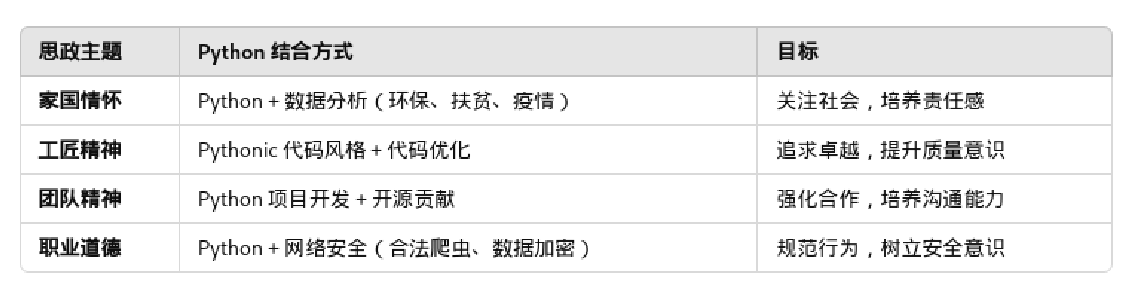
\includegraphics[width=0.9\linewidth]{policy.eps}
		\end{center}
	\end{figure}
	\pause
	不同思政目标所对应的实现方式
	\begin{center}
		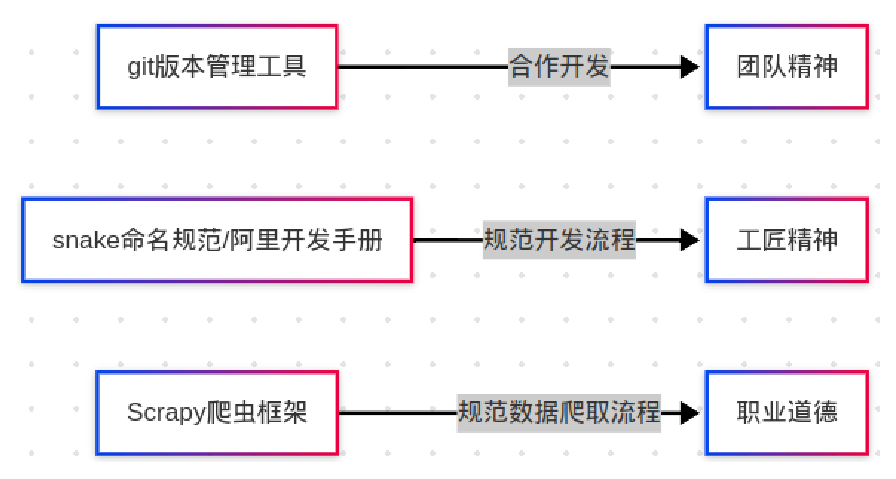
\includegraphics[width=0.5\linewidth]{tools_for_policy.eps}
	\end{center}
\end{frame}


\section{本节内容概述}



\section{容器}

\subsection{元组}

\begin{frame}
	\frametitle{元组}
	\framesubtitle{创建元组}
	\begin{block}{definition}
		元组是有序的、\red{不能更改的}、可重复的容器。
	\end{block}
	\pause
	\begin{block}{example}
		创建元组thistuple = ("apple", "banana", "cherry", "apple", "cherry")
		使用构造器创建元组thistuple = tuple(("apple", "banana", "cherry", "apple", "cherry"))
	\end{block}
	\pause
	\begin{alertblock}{定义单个元素的元组}
		创建单元素的元组必须在元素后添加逗号
		thistuple = ("apple",)
		print(type(thistuple))
		thistuple = ("apple")
		print(type(thistuple))
	\end{alertblock}

\end{frame}
\begin{frame}
	\frametitle{元组}
	\framesubtitle{访问元组}
	\begin{itemize}
		\item 索引(正向,反向,截取)
		\item 遍历
		\item 筛选
	\end{itemize}
\end{frame}

\begin{frame}
	\frametitle{元组}
	\framesubtitle{添加元素/删除元素}
	因为tuple是不可更改的,如果需要更改tuple中的元素需要将其转化为list类型的变量

\end{frame}

\begin{frame}
	\frametitle{元组}
	\framesubtitle{解包}
	将元组中的元素一次赋给多个变量
	\begin{block}{example}
		fruits = ("apple", "banana", "cherry", "strawberry", "raspberry")

		(green, yellow, *red) = fruits

		print(green)
		print(yellow)
		print(red)
	\end{block}
\end{frame}
\begin{frame}[t]
	\frametitle{元组}
	\framesubtitle{方法}
	\begin{itemize}
		\item count() :输出某个元素在tuple中出的次数
		\item index() :输出某个元素在元组中第一次出现位置的索引值
	\end{itemize}

\end{frame}

\subsection{集合}

\begin{frame}[t]
	\frametitle{集合set}
	\framesubtitle{set创建}
	\begin{block}{definition}
		集合是无序、\red{不可更改}、不可重复、无索引的容器.(不可更改🈯的是集合元素的值无法更改,但不影响集合本身添加删除元素)
	\end{block}
	\pause
	\begin{block}{example}
		thisset = \{"apple", "banana", "cherry"\}
		print(thisset)
		通过构造器创建set thisset = set(("apple", "banana", "cherry")) # note the double round-brackets
	\end{block}
	\pause
	\begin{alertblock}{set元素不允许重复}
		thisset = \{"apple", "banana", "cherry", True, 1, 2\}\\1和true在set中被认为是值相同的元素
		print(thisset)
	\end{alertblock}
\end{frame}
\begin{frame}[t]
	\frametitle{集合}
	\framesubtitle{访问set}
	\begin{itemize}
		\item<1-> 索引
			\pause
			\begin{block}{example}
				list({1,2,3})[2]
			\end{block}
			\pause
		\item<2-> 遍历
			\pause
			\begin{block}{example}
			for item in {1,2,3}:
			\end{block}
			\pause
		\item<3-> 筛选
			\pause
			\begin{block}{example}
				[item for item in {1,2,3} if item > 2]
			\end{block}

	\end{itemize}
\end{frame}

\begin{frame}[t]
	\frametitle{集合}
	\framesubtitle{向集合中添加元素}
	\begin{itemize}
		\item add()
		\item update()更新原集合、union()=|返回新集合
	\end{itemize}
\end{frame}

\begin{frame}[t]
	\frametitle{集合}
	\framesubtitle{删除集合中的元素}
	\begin{itemize}
		\item remove():删除指定值的元素,若值不存在报错

		\item discard():删除指定值的元素,不报错

		\item pop():随机删除元素
		\item clear():清空元素
	\end{itemize}
\end{frame}
\begin{frame}[t]
	\frametitle{集合}
	\framesubtitle{对集合的操作}
	\begin{center}
		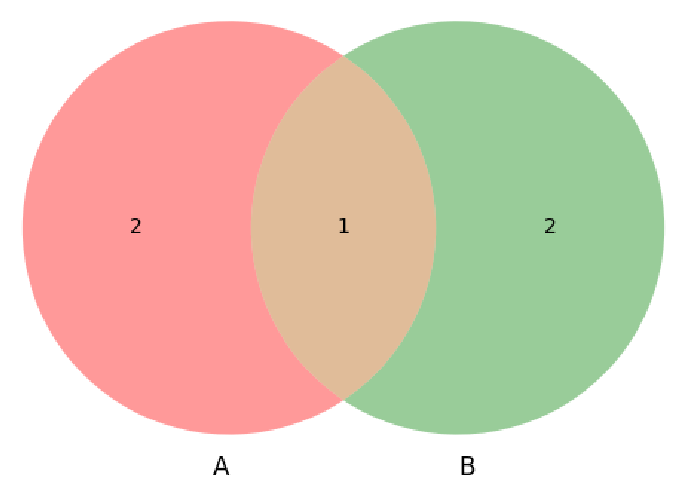
\includegraphics[width=0.4\textwidth]{venn_diagram.eps}
	\end{center}
	\begin{itemize}
		\item intersection()   将两集合中所有重复的元素返回到新集合,取得1
		\item difference()	将在另一个集合中出现过的元素筛掉形成新集合,取得A2或B2
		\item symmetric\_difference()  两个集合中所有差异的元素全部同步到新集合,取得A2 和 B2
	\end{itemize}

\end{frame}

\subsection{字典}

\begin{frame}[t]
	\frametitle{字典}
	\framesubtitle{创建字典}
	\begin{block}{definition}
		字典是有序、可改值、不允许出现重复的键
	\end{block}
	\pause
	\begin{block}{example}
		thisdict = \{
		"brand": "Ford",
		"model": "Mustang",
		"year": 1964
		\}\\
		thisdict = dict(name = "John", age = 36, country = "Norway") :使用构造器创建集合\\
		dict.fromkeys(Iterable, default\_values):快速构造默认值相同的字典
	\end{block}

\end{frame}
\begin{frame}[t]
	\frametitle{字典}
	\framesubtitle{字典元素的访问}
	\begin{itemize}
		\item get():通过key值访问某个元素的value
		\item keys():返回所有的keys
		\item values():返回所有的values
		\item items():返回所有的items
		\item 遍历字典
		      \begin{itemize}
			      \item for x in dictionary 和keys():遍历keys
			      \item for x in dictionary: dictionary[x] 和values()便利values
			      \item for x,y in dictionary.items: 遍历(key,value)
		      \end{itemize}

	\end{itemize}
	\begin{alertblock}{Attention}
		x =dictionary.keys():在获取字典的keys之后任何对字典的修改都会同步到keys列表,valuse和items也类似
	\end{alertblock}

\end{frame}
\begin{frame}[t]
	\frametitle{字典}
	\framesubtitle{向字典中添加元素}
	\begin{itemize}
		\item dictionary[keys]=values
		\item update(): 函数的值可以是任何iterable类型的变量
	\end{itemize}

\end{frame}
\begin{frame}[t]
	\frametitle{字典}
	\framesubtitle{删除字典中的元素}
	\begin{itemize}
		\item pop(key):删除指定key的元素
		\item popitem():删除最后一个元素
		\item clear():清空字典
	\end{itemize}
\end{frame}
\end{document}
